% Chapter 4: DISCUSSION

\chapter{Discussion} % Main chapter title

\label{discussion} % For referencing the chapter elsewhere, use \ref{Chapter1} 

%%----------------------------------------------------------------------------------------
%
%% Define some commands to keep the formatting separated from the content 
%\newcommand{\keyword}[1]{\textbf{#1}}
%\newcommand{\tabhead}[1]{\textbf{#1}}
%\newcommand{\code}[1]{\texttt{#1}}
%\newcommand{\file}[1]{\texttt{\bfseries#1}}
%\newcommand{\option}[1]{\texttt{\itshape#1}}

%----------------------------------------------------------------------------------------

%PUT RESULTS IN BROADER PICTURE

%* What informed choice of methods?
%* Could it have been done in another way?
%* Which aspects of the work could be taken further?


%----------------------------------------------------------------------------------------
%----------------------------------------------------------------------------------------
\section{Validation on more images}\label{sec:validation}

%[INSERT ERROR MEASUREMENTS NEED TO BE OBTAINED, CURRENTLY NOT EXISITING IN MANUALLY COMPUTED ANGLES AND ALSO NOT IN ROOTSKEL, IN ORDER TO MAKE VALID ASSUMPTIONS ON ROBUSTNESS AND REPITABILITY]

Certainly, validation needs to be done on a bigger data set in order for our claims to be valid.
%not only be a well grounded belief.
As this could not happen in this project due to time constraints we suggest a thorough (statistical) analysis of the collected data and, subsequently, quantification of population heterogeneity in electrotropic responses as future work.

Obtaining standard deviations in the measurements, both in the manual and the computational method, are necessary to make claims on their precision and therefore robustness of \textit{RootSkel}. Quantifying accuracy is almost impossible without having some underlying model or valid assumptions as we do not know the true theoretical values, and any measurements will inevitably contain errors, a problem also identified in \cite{dee2015image}.
% This makes comparing it to the manual angles difficult
% Of course, we are now left with the problem of defining reasonable accuracy versus people: if someone is measuring plants manually, are they sure they are measuring the right thing?. 

%Of course, we are now left with the problem of defining reasonable accuracy versus people: if someone is measuring plants manually, are they sure they are measuring the right thing?
%WE NEED TO FIT AGAINST STH TO SHOW THAT ACCURATE

%FROM ROOTTRACE: IT IS NOT NECESSARY FOR THOSE WISHING TO USE ROOTTRACE TO UNDERSTAND THE UNDERLYING METHODS IN GREAT DEPTH; HOWEVER, THE INFORMATION IN THIS SECTION MAY HELP THOSE INTERESTED TO UDNESTAND THE SITUATIONS IN WHICH IT CAN BE APPLID AND WHAT CAN CAUSE THE SOFTWARE TO FAIL.
%FURTHER TECHNICAL DETAILS ABOUT ROOT TRACE'S EARLY DEVELOPMENT CAN BE FOUND IN PREVIOUS WORK. LOG FILES CAN BE FOUND IN....

%----------------------------------------------------------------------------------------
%----------------------------------------------------------------------------------------
\section{Challenges and limitations of \textit{RootSkel}}

%Difficult decisions had to be made in planning the research, leading to subsequent tradeoffs. Then, focus in on the need for future work.
During the development process of \textit{RootSkel} various challenges were encountered and trade-offs to overcome them were necessary; there are some limitations of \textit{RootSkel} that users should be aware of and future developers can work on.


%----------------------------------------------------------------------------------------
\subsection{Non-planar roots}

Another challenge of studying electrotropism compared to gravitropism in an agar gel is that it is much harder to keep the roots in a plane, i.e. keep them from growing in a third direction, due to the experimental set up to capture electrotropic responses. Since we only take 2D images, there will inevitably be an error in the angle calculation by the simple fact that the plants do not bend in a perfect plane.
%compared to gravitropism, it is much harder to keep the roots in a plane. we only capture the angle based on 2D images.


%----------------------------------------------------------------------------------------
\subsection{Skeletonisation of the root}

The biggest challenge in the development process was to extract the root skeleton, precisely to discern the root from the background and the noise, mainly due to the low contrast. % between them.
Our approach of implementing different colour and intensity filters is not optimal as these might not filter out the noise. 
%For that we mostly implemented colour and intensity filters which can still include different kinds of noise. 
The most distinct feature of the root is the tubular structure and functions that recognise this have been used; however, this can still be optimised in the future. 

%we did not get the most out of it
%get rid of loop

For the angle calculation it is important that the tip of the root is included in the skeleton. This has shown to be particularly challenging in Arabidopsis images as the root often appears translucent \cite{french2009high} and causes algorithms to fail \cite{french2009high}. Where some tools require some backround appearance statistics or parameter as input from the user \cite{french2009high}, \textit{RootSkel} offers a separate optional step \textit{Force tip} for the user to trace along the tip of the root. Increasing the contrast is expected to help tremendously to detect the root tip; equally for other methods \cite{french2009high}.


%%----------------------------------------------------------------------------------------
%\subsection{Challenging images}\label{subsec:challengingImages}
%
%%There is a very low contrast between the background and the roots, so that one could hardly recognise the roots on some images [INSERT EXAMPLE IMAGE HERE].
%The data set we were working on contained highly challenging images (see figure \ref{fig:challenginRoots}), this was due to
%\begin{itemize}
%	\item Low contrast between roots and background; the roots were almost not discernible for the human eye without previous treatment of the image (see subfigure \ref{figsub:lowContrast})
%	\item Lots of noise or objects that we classified as noise as there was no apparent structure to it (see subfigure \ref{figsub:noisy})
%	\item Different noise patterns, i.e. inconsistency, across the images; the noise was subtle or hiding and could only made visible on filtered images (see subfigure \ref{figsub:noisy})
%	\item Numerous objects that were of no interest, especially the ones interfering with our object of interest (see subfigure \ref{figsub:stickyObject})
%	\item Low resolution of the images or object of interest itself taking up only a small fraction of the whole image. 
%\end{itemize}
%Highly pixeled images made not only the preprocessing but especially the curvature computing part challenging; also various MATLAB functions do not work well on sparse data.
%In section \ref{futuredataAquis} we make suggestions for future data collection.
%
%\begin{figure}[H] 
%	\begin{subfigure}[b]{0.5\linewidth}
%		\centering
%		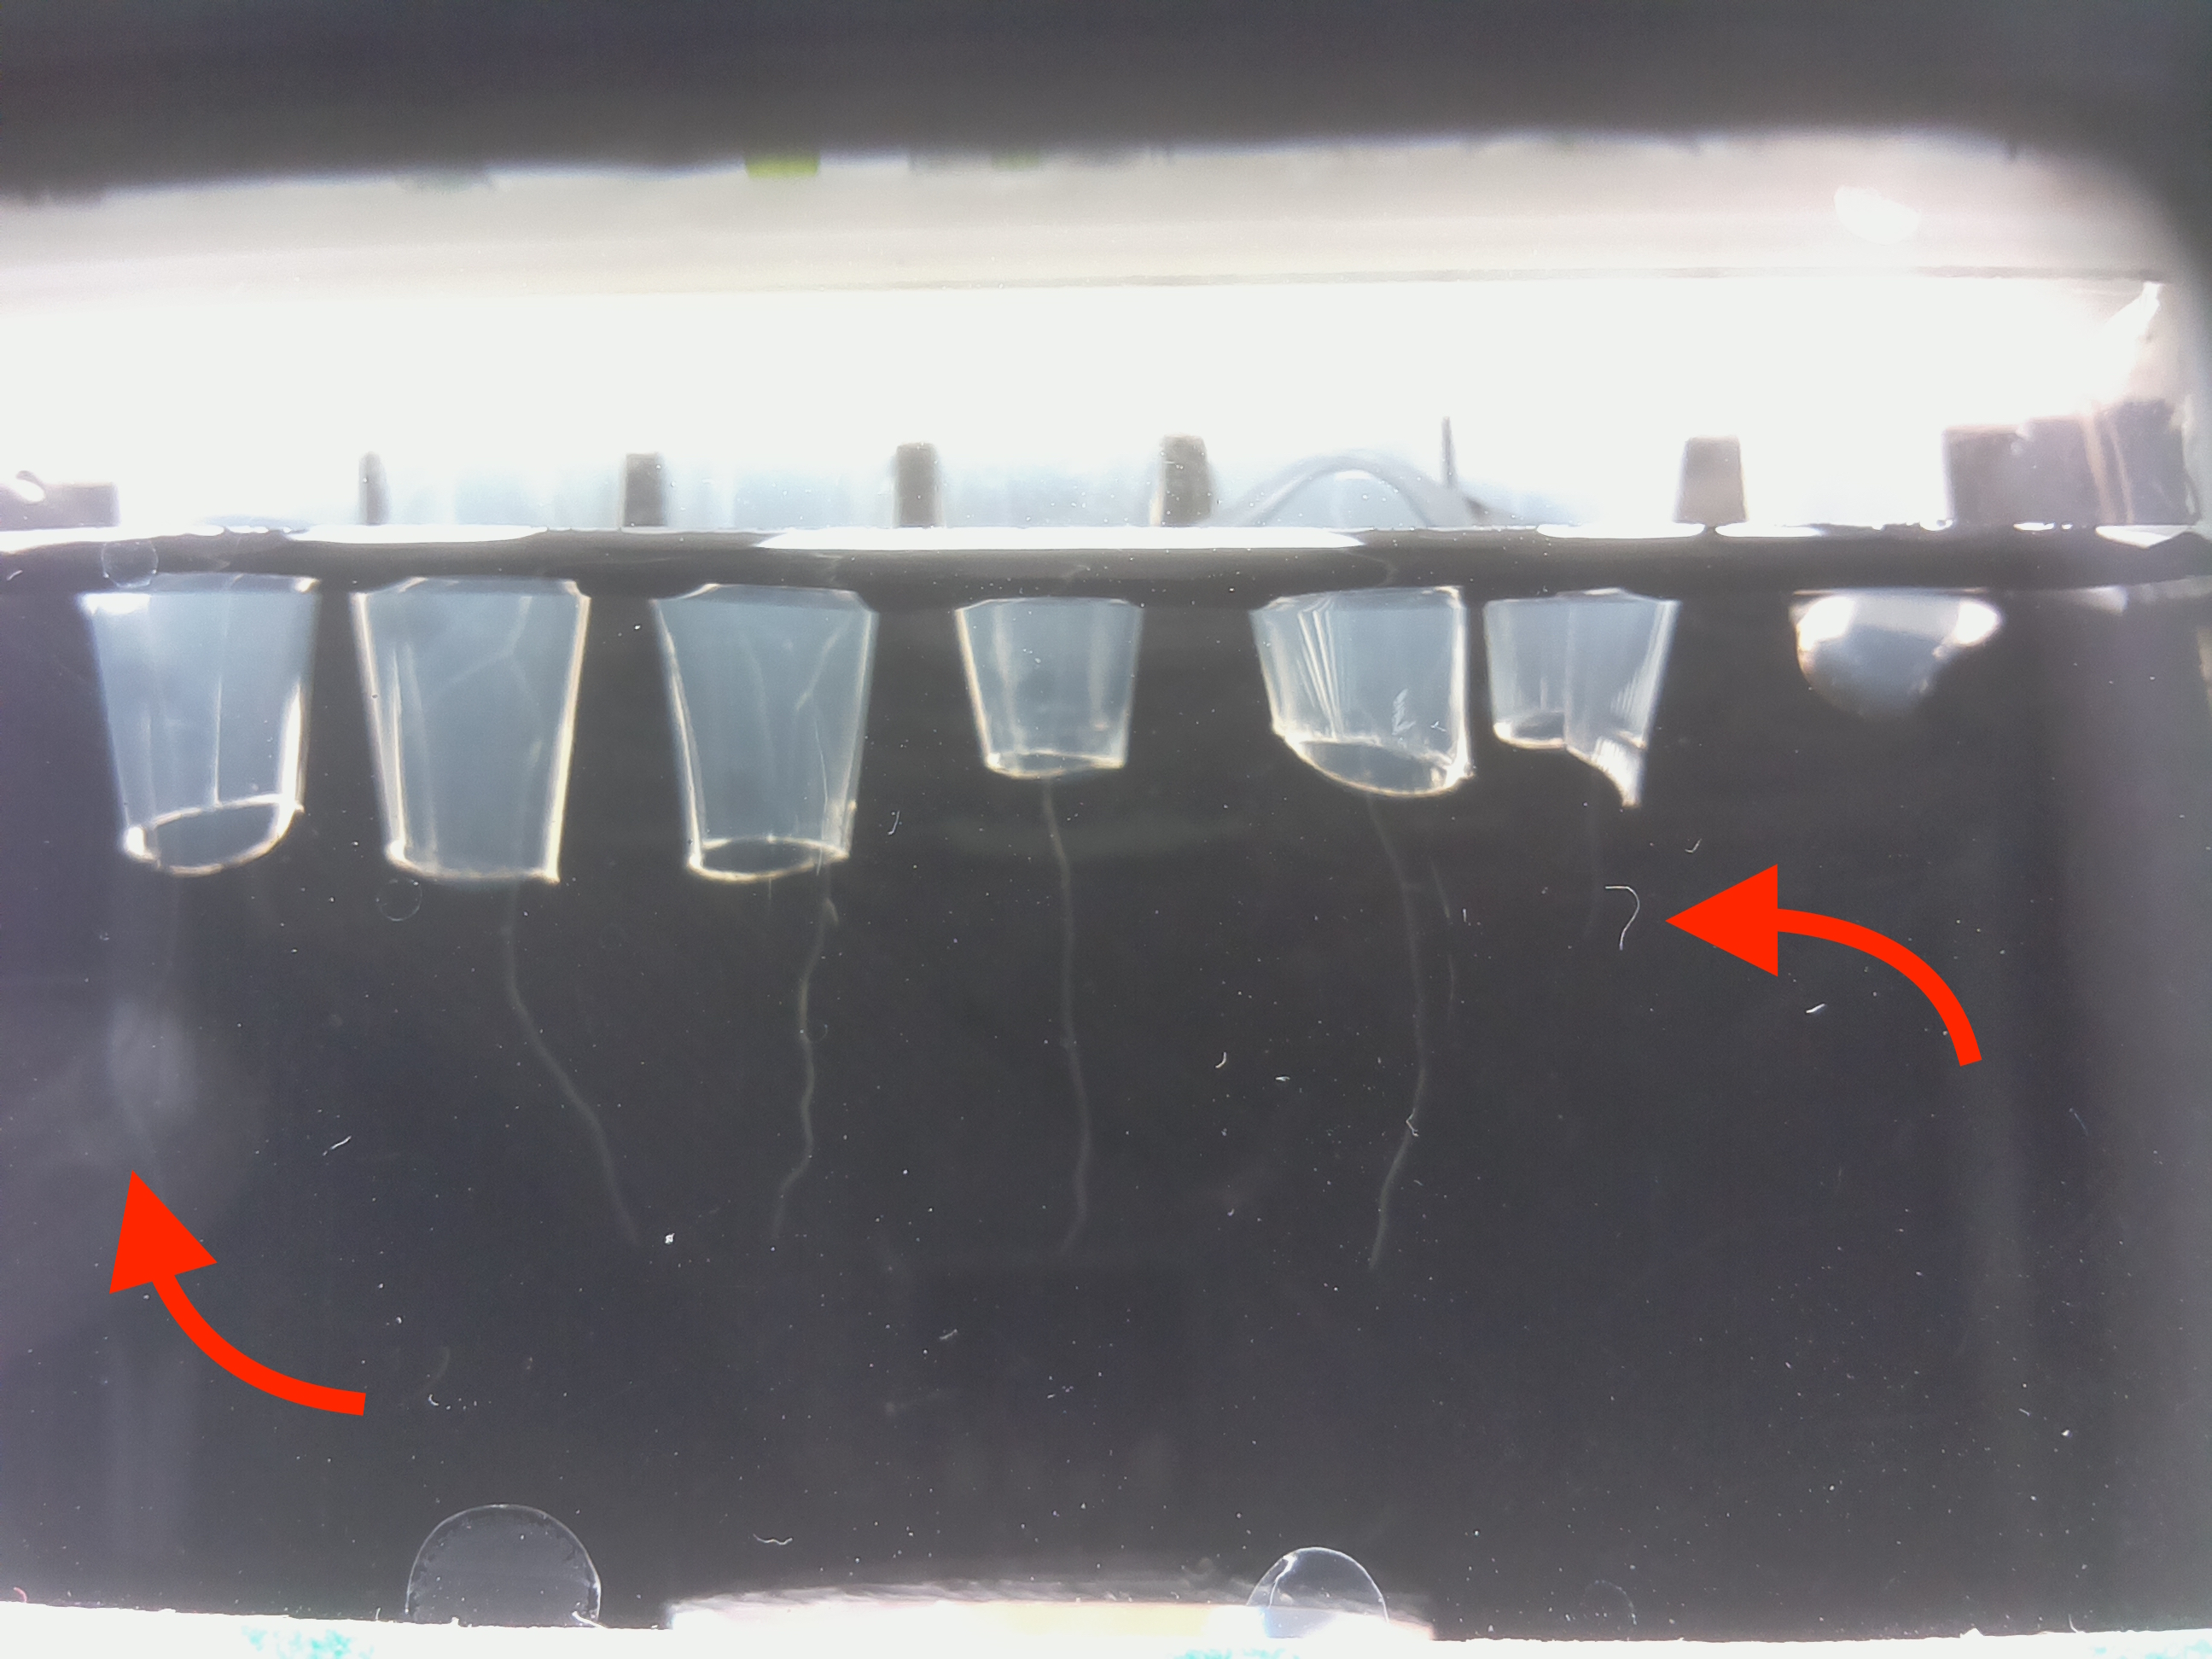
\includegraphics[width=0.75\linewidth]{2018-03-08_1000.jpg} 
%		\caption{Changing light reflection (root on the LHS\\ is lost), low contrast} 
%		\label{figsub:reflection} 
%		\vspace{4ex}
%	\end{subfigure}%% 
%	\begin{subfigure}[b]{0.5\linewidth}
%		\centering
%		\includegraphics[width=0.75\linewidth]{2018-02-28_2030.jpg} 
%		\caption{Foreign object sticking to root, \\blurry regions, other objects} 
%		\label{figsub:stickyObject} 
%		\vspace{4ex}
%	\end{subfigure} 
%	\begin{subfigure}[b]{0.5\linewidth}
%		\centering
%		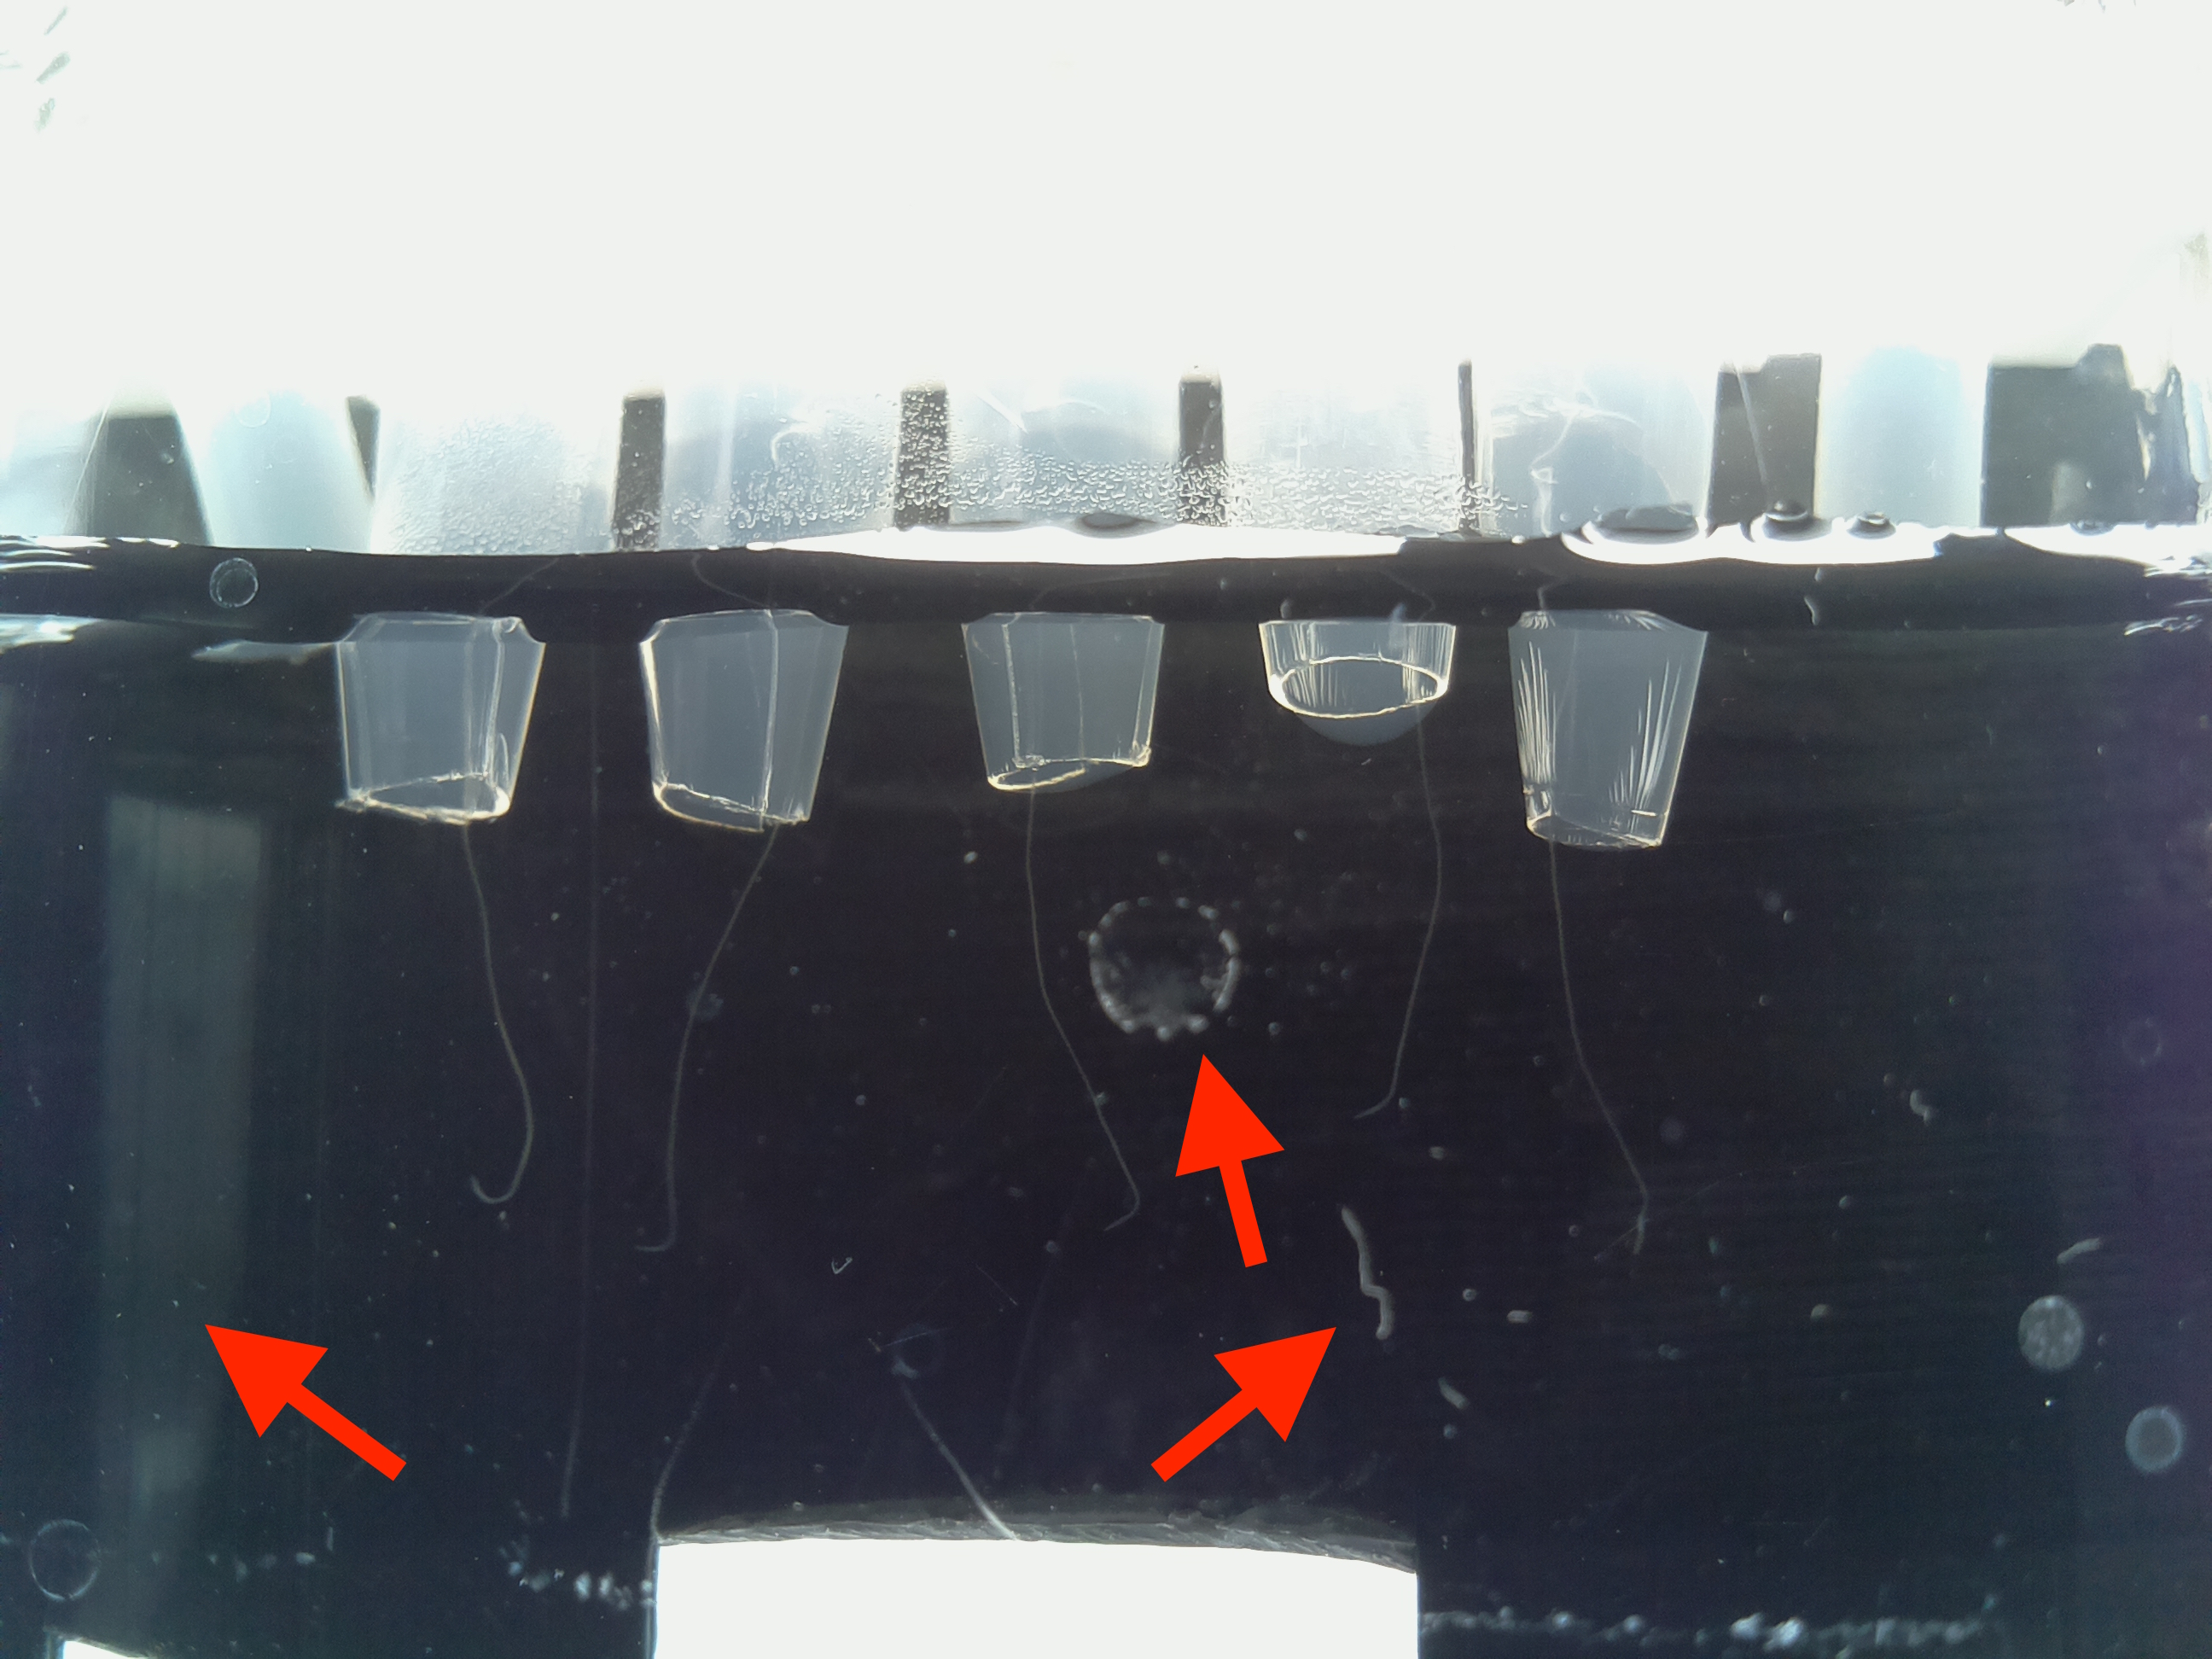
\includegraphics[width=0.75\linewidth]{2018-04-24_1840.jpg} 
%		\caption{Noisy image, many objects of same colour} 
%		\label{figsub:noisy} 
%	\end{subfigure}%%
%	\begin{subfigure}[b]{0.5\linewidth}
%		\centering
%		\includegraphics[width=0.75\linewidth]{2018-03-06_2000.jpg} 
%		\caption{Low contrast, roots touching each other} 
%		\label{figsub:lowContrast} 
%	\end{subfigure} 
%	\caption{Problems of images; images taken from our data set: (A) 2018-03-08\_1000.jpg, (B) 2018-02-28\_2030.jpg, (C) 2018-04-24\_1840.jpg, (D) 2018-03-06\_2000.jpg}
%	\label{fig:challenginRoots} 
%\end{figure}


%Eg specs not so much of an issue as separate from the root. Issue when it is connected.


%----------------------------------------------------------------------------------------
\subsection{Scalability and reproducibility}

The variation in the noise pattern in the images (see \ref{fig:challenginRoots}) made it difficult to automate the process of extracting the root skeleton; every image is unique and needs to be treated uniquely. The developed pipeline works well on many images; other images require special and longer treatment. Scalability has been and continues to be a challenge.

%Many iterations on different images of our data set led to an elaborate tool for the pre-processing of the roots; however, we cannot prevent the tool from failing on some images. 
Even though our angle computation is deterministic %and straight-forward 
and only depends on the root skeleton, there is still some variability in the preprocessing step due to the user's input. This means, it can happen that for the very same root in the very same image we get slightly different angles due to slightly different root skeletons. %This is due to the fact that our current version of \textit{RootSkel} does require user input for the preprocessing steps, meaning results of the root skeleton might slighly vary depending on the user's input.
However, the error in the angles we observed is tiny and within reasonable bounds to be negligible; we expect the measurement error to be much smaller than in the manual computations. Having said that, reproducibility can not be fully guaranteed. %; errors should be quantified for each of the methods to make a valid claim regarding robustness and actual improvement in the angle computation. 
%INSERT ERROR COMPUTATION NECESSARY, SHOW THAT OUR METHOD IS MORE ROBUST, LESS MEASUREMENT ERROR/ CLOSER TO THE TRUE THEORETICAL VALUE THATN NECESSARY



A major disadvantage of the bottom-up approach (see \ref{sec:workflow}) is that errors can accumulate: one wrong result made by one process commonly introduces further errors later in the pipeline and in the worst case can seriously affect the final results \cite{pound2013rootnav}.
% In the worst cases, this can initiate a cascading effect that can seriously affect final results. Poor noise reduction can lead to thresholding errors, for example. Imperfect thresholding in turn disrupts skeletonization, adding spurious segments and introducing breaks into true roots. 

Possible solutions are more interactive tools that allows the user to clean up and correct these results \cite{armengaud2009ez,clark20113} like the optional steps in \textit{RootSkel}. Manual corrections to refine the results can be frustrating but should in general be preferred to inaccurate or unprecise manual. calculations.

For \textit{top-down} approaches a model of the object of interest is needed; this could be of topological or geometrical nature \cite{pound2012cellset} or a number of assumptions \cite{mooney2012developing}. In our case we could focus the attention to the tubular structure of the root, the unique proerty of the roots. Top-down approaches tend to be more easily adapted to a wider range of data but require a suitable model a priori  \cite{pound2013rootnav}.


%\cite{pound2013rootnav}:
%One response to this problem is to quantify only broader root measures, such as convex hulls or overall root depth (Galkovskyi et al., 2012), which do not require detailed descriptions of the root architecture (nested structure, emergence angles, etc.). The alternative is to provide interactive tools (Armengaud, 2009; Clark et al., 2011) that allow the user to clean up and correct automatically generated results. This can be hard to achieve satisfactorily when large corrections are needed. More importantly, though most users are willing to spend some time interacting with their data to refine results, manual correction of obvious errors can be frustrating and requires the user to carefully scrutinize all of the automatically reported results. It tends to reduce both the confidence in, and use of, tools that rely upon it excessively. THEREFORE, CLEAN DATA THE MORE IMPORTANT
%By contrast, top-down approaches match a clearly stated model of the object(s) of interest to the input data. Models may be explicit topological or geometrical structures, such as the network of contours employed by CellSet (Pound et al., 2012) or a loose collection of assumptions embedded in a search process (Pridmore et al., 2012). Though requiring a suitable model to be identified a priori, top-down methods can be more resistant to global image clutter and intensity change (French et al., 2009). The top-down approach focuses attention on the properties of target objects, roots, rather than on the properties of images of roots. As a result, top-down methods are frequently applicable, or at least more easily adapted, to a wider range of data sets.




%COMMENTED OUT DUE TO WORD COUNT
%%----------------------------------------------------------------------------------------
%\subsection{High user-interaction}
%
%Even though \textit{RootSkel} comes with a lot of flexibility and simplicity in the user interaction, it would be desirable to have less user input to guarantee reproducibility and save time in the process overall. 
%
%This might overall be improved by images of higher quality in the future as well as implementing approaches that try to automate the whole preprocessing process.



%Might be reduced with better-quality images, however very flexible.


%standard-deviation not as high as i think?

%Would be desirable if it could be automated more. 

%%----------------------------------------------------------------------------------------
\subsection{Other tools and languages}

Even though MATLAB has several advantages, it might be worth looking into alternative non-proprietary programming languages to make the tool accessible to a wider public or other options of making the tool portable, i.e. without requiring the user to have MATLAB installed.
Alternative languages one might want to consider are \textit{Julia} and \textit{Python}. Another recommended language is \textit{OpenCV} as it is very fast and well documented.

It might be worth looking into \textit{PlantCV} to create image processing pipelines for plants; it offers several image processing packages designed for plant biology research in Python syntax and is built upon open-source software platforms like OpenCV, NumPy and MatPlotLib \cite{plantCV}. It also points out some key things to consider when generating the data; more on that in section \ref{futuredataAquis}.

Other non-open source software such as \textit{ImageJ}, a Java based image processing program, and \textit{Avizo} which is a general-purpose commercial software application for scientific and industrial data visualisation and analysis with a nice GUI, were not investigated further in this work. 

 
%----------------------------------------------------------------------------------------
%----------------------------------------------------------------------------------------
\section{Further work}

In the following we will outline suggestions for future work including things that need optimisation or features that might be nice to implement in the future. 

%COMMENTED OUT DUE TO WORD COUNT, see point below
%%----------------------------------------------------------------------------------------
%\subsection{Use more shape-based filters}
%
%To overcome the problem of separating the root from the background and the noise, one should use and optimise specific shape-based filters [AS USED IN.. INSERT REFERENCE HERE] instead of a series of colour and intensity filters that have shown to be not very efficient on our data set. This is due to the observation that the tubular structure is the most distinctive feature of the roots. Tubular structure recognising filters have been implemented but there is room for improvement. This might help to extract the skeleton more easily and reliably without the need of optional cropping or cleaning.


%%----------------------------------------------------------------------------------------
%\subsection{Effective noise reduction}
%
%In order to tackle the problem of noise reduction, it might be advisable to consult an expert not only on image processing but especially in the field of noise reduction to effectively implement filters that get rid of the noise our images contain. 
%
%%COMMENTED OUT DUE TO WORD COUNT
%%To overcome the problem of separating the root from the background and the noise, one should use and optimise specific shape-based filters [AS USED IN.. INSERT REFERENCE HERE] instead of a series of colour and intensity filters that have shown to be not very efficient on our data set. This is due to the observation that the tubular structure is the most distinctive feature of the roots. Tubular structure recognising filters have been implemented but there is room for improvement. This might help to extract the skeleton more easily and reliably without the need of optional cropping or cleaning.
%
%%EXPLOIT FACT THAT TIME SERIES IMAGE


%----------------------------------------------------------------------------------------
%\subsection{Less user input up to automatisation}
\subsection{High-throughput and robustness}

Here in the first version of \textit{RootSkel}, the main goal was to standardise the angle computation. If in the future  a method for handling the different noise patterns in the images was efficiently handled which required less user input; it would be desireable to automate the whole angle computation. Indeed, robust high-throughput techniques for plant image processing problems have been desired for very long \cite{hartmann2011htpheno,diener2013automated,lee2018automated,plantCV} but have proven to be very difficult due to the challenges outlined above.

%In order to tackle the problem of noise reduction, it might be advisable to consult an expert not only on image processing but especially in the field of noise reduction to effectively implement filters that get rid of the noise our images contain. 

%in order to increase robustness on unseen data (which was not the goal of this work), first, one needs to collect high-quality data and second, tweak the data 

%REFER TO ML APPRAOCHES: \cite{pound2017deep}


%----------------------------------------------------------------------------------------
%\subsection{Robustness}

%The workflow developed via  many iterations on different images and 
%elaborate pre-procecessing tool for skeletonisation
%high functionality, reiterated process
%has been overengineered on one dataset, if it should be robust on other data, it needs to be trained/ tweeked on other data.



It would be desirable to make the tool more robust so it will work on unknown and other type of data (which was not the goal of this work) and to make the tool available to a wider public. For that, one might want to first and foremost collect higher quality images in the future (for suggestions on data collection (see \ref{futuredataAquis}) and second, investigate automated approaches. % such as adaptive thresholding. 
Our specific problem was not found to benefit immediately from having machine learning applied to it; however, in slightly different contexts deep learning could be a rich avenue to explore in order to discover patterns in the data \cite{pound2017deep,lee2018automated}.

%High-throughput software tools that can produce objective, quantitative analyses od the resulting images are now required.



%COMMENTED OUT DUE TO WORD COUNT
%%----------------------------------------------------------------------------------------
%\subsubsection{Adaptive thresholding}
%%  Another similar approach would be to ask the user to quickly draw small ROI (rectangles) to frame each root in the inverted (much easier) image. The code could then global threshold each ROI separately and go from there.
%Before opting to take user input in the form of samples of the roots in the image, we investigated adaptive (global) thresholding on each of the root and an adaptive variable setting approach on all of the roots together to extract the root. This however failed, or would have been beyond the scope of this project. % -- the reason why we implemented a user-centric approach.
%%the way it was suggested.


%COMMENTED OUT DUE TO WORD COUNT
%%----------------------------------------------------------------------------------------
%\subsection{Maintenance and bug fixing}
%
%Even though \textit{RootSkel} is a tool that is ready to be used, and we tried to cover as many cases as possible of things that could go wrong, on some exceptional images the tool might still exhibit bugs that need fixing.
%As we commented the code generously and kept log files about all changes and decisions made, a future developer should not have any problems building upon our source code.

%INSERT BUG FIXES HERE


%COMMENTED OUT DUE TO WORD COUNT
%%----------------------------------------------------------------------------------------
%\subsection{More features}
%
%More features such as a zooming in function at the beginning of force tip can be included; however, they will not change anything in the core functionality of \textit{RootSkel}.
%
%%WE HAVE INCLUDED THAT IN THE CURRENT VERSION ALREADY
%%Also, what would be nice to implement in the GUI or in an extra window from a user perspective is a graph superimposing the skeleton to illustrate which angle is computed. This way, the user can doublecheck that the correct angle is computed. This feature will be provided in the next version of \textit{RootSkel}.


%COMMENTED OUT DUE TO WORD COUNT
%%----------------------------------------------------------------------------------------
%\subsection{Other ways of curvature and angle measuring}
%
%%SHOULD WE REALLY INCLUDE THAT?
%%What was implemented as we found that this approach worked best on these data and this resolution. However, MATLAB does have some issues with singularities, e.g. whenever the angle is (exactly) 45 degrees one should doublecheck if this is due to an infinity issue in the arctan. 
%
%For the future, we might want to exploit the fact that we have time series data for the angle computation. This means that technically, it does not require the computation of the angle in each single image but only the difference in the angle to the previous image, since we assume the turning point does not change over time. 
%
%Once we have higher-resolution images or a denser data set, we will also  achieve a better approximation of the real curvature. In the meantime, it might be worthwhile to investigate more maybe better approaches to compute curvatures on sparse data sets. 
%
%Also, alternative definitions instead of an emulation of the so far manually computed angle, such as the curvature itself and possibly more robust methods of computing it might be worth further looking into. 
 

%----------------------------------------------------------------------------------------
%\subsubsection{Curvature better on dense data set}
%
%% FUTURE WORK: curvature on a sparse polygon like this might not be very
%% meaningful but that does not mean it is not possible to apply the
%% discrete approximation to the derivative to compute it. 
%% The same code on a more densly samples outline will give a good
%% approximation of the curvature of the outline
%
%%Standardised and automated version of angle computation



%%%%%%%%%%%%%%%%----from here

%----------------------------------------------------------------------------------------
\subsection{Error quantification in the angle computation}

Another additional step towards validation or an integral part of taking measurements in general %and especially precision 
%to ensure repeatability of our results 
%would be to include 
is to quantify the error in the angle computation, e.g. the maximum or average error in the final result due to the changes in the pre-processing step. %This could be computed 
One can try to do achieve this empirically by trying our tool on a large amount of data to estimate the statistical error; there are ways to also try to quantify the instrumental error. 
%THIS WORK HAS STARTED ALREADY.


%COMMENTED OUT DUE TO WORD COUNT, maybe in appendix? --- DO INCLUDE IF WE STILL HAVE WORDS LEFT
%%%----------------------------------------------------------------------------------------
%\subsection{Other programming languages}
%
%Even though MATLAB has several advantages, it might be worth looking into alternative non-proprietary programming languages to make the tool accessible to a wider public or other options of making the tool portable, i.e. without requiring the user to have MATLAB installed.
%Alternative languages one might want to consider are \textit{Python} and \textit{Julia}. Another recommended language is \textit{OpenCV} as it is very fast and well documented. Other non-open source software such as \textit{ImageJ}, a Java based image processing program, and \textit{Avizo} which is a general-purpose commercial software application for scientific and industrial data visualisation and analysis with a nice GUI, were not investigated further in this work. 


%%%%%%%%%%%%------------------------------------------
%
%errors should be quantified for each of the methods to make a valid claim regarding robustness and actual improvement in the angle computation. 
%
%Only if the measurement errors in our 
%
%HOW QUANTIFY THAT REALLY CLOSER TO THEORETICAL VALUE. REALLY NEED .
%
%TRY TO FIT IT TO A PHYSICAL MODEL/ UFNCTION/ MEASNURE, MAKE SOME CLAIMS BASED ON A NUMBER OF ASSUMPTIONS. 
%ANY PARTICULAR VALUE IS NOT INTERESTED, OUT OF CONTEXT DOES NOT HELP US MUCH. 
%
%
%ONLY SHOW THAT PRECISE, NOT ACCURATE.
%
%WE NEED TO FIT IT AGAINST STH TO SHOW THAT ACCURATE.
%
%PRECISION IS REPEATABILITY. ACCURACY -- HOW CLOSE TO TRUE VALUE.
%
%SAY STH ABOUT PRECISION, NOT ABOUT ACCURACY
%SINCE WE HAVE NO REAL THEORETICAL VALUE
%
%
%errors should be quantified for each of the methods to make a valid claim regarding robustness and actual improvement in the angle computation. 
%
%
%WHOM IS CLOSER?
%TRY TO FIND OUT WHO IS CLOSER, WITHOUT KNOWING THE TRUE VALUE. 
%IN A PITCHBLACK ROOM WITHOUT TOUCH. IF YOU DONT KNOW WHERE THE GOBLET. 
%WE DO NOT KNOW WHICH ONE IS CLOSER TO THE TEAPOT (RUSSELS TEAPOT, burden of the proof lies with person making the claim)
%
%RUSSELS TEAPOT
%
%
%
%YOU NEED ERRORS TO SAY STH, OTHERWISE THE VALUES ARE MEANINGLESS.
%HOW CAN QUANTIFY THESE ERRORS?
%
%WORK TOWARDS PRECISION USING STANDARD DEVIATION 
%HELPS TOWARDS MEASUREMENT ERRORS, QUANTIFIE ABILITY OF MACHINE/PERSON. BUT OTHER FACTORS WHICH WE ARE NOT GOING TO TOUCH,  USING EYES, HANDS/ MOUSE.
%
%HOW TO KNOW REAL VALUE?
%ERRORS JUST SAY STUFF ABOUT MEASUREMENTS. 
%
%
%CAN'T COMPUTE ACCURACY, WE SIMPLY DON'T KNOW TRUE THEORETICAL VALUE.
%HOW CAN A MODEL LOOK LIKE IN THIS CASE?


%NICK:
%We know that my measurements contain (sometimes quite large) degrees of error, but we also know they are going to be accurate enough that they represent roughly what the root is doing. So if the root is fully aligned with the field the measurement I take should be close to 0°, if it's only made it half of the way it should be close to 45°. 
%
%
%
%This means that we can use the measurements I have taken as a guide to make sure that your computed angles are in the right sort of range to reflect what is actually happening in the experiments. 
%
%
%In terms of computing the "improvement of the angle computation", if I understand this correctly, I am not sure how you would do this and actually I'm not sure that you need to. It is much more important for us to get a product that can improve the reproducibility of our measurements (especially between different users) as opposed to something that will measure the root angles more accurately vs manual measurements. 
%
%
%%%%%%%%%%%%------------------------------------------

%----------------------------------------------------------------------------------------
%----------------------------------------------------------------------------------------
\section{Broader application of \textit{RootSkel}}

This software tool can be reused for many purposes and is not restricted to root detection.
It might also be used for "easier" problems like analysing gravitropism.

